\chapter{Dataset Reconstruction}
\label{cha:3}

\section{BAT dataset} \label{bat-characteristics}

The BAT dataset \cite{spinde-2023-bat} is selected for this project due to its suitability for article-level analysis (contains titles, URLs of articles, and outlet information) and better labelled with reliability score instead of binary label or political alignment (left, right). The dataset contains 6345 rows of manually labelled news articles from 255 English-speaking news outlets (US-based), originally scraped from Ad Fontes Media's website along with their respective \textbf{political bias} and \textbf{reliability scores}. Articles in the dataset encompassed a wide range of topics such as COVID-19, politics, and lifestyle. The political bias score measures the extent of political influence, ranging from -42 (most extreme left) to +42 (most extreme right). The reliability score reflects the article's truthfulness, with values ranging from 0 (least reliable, containing inaccurate or fabricated information) to 64 (most reliable, original fact reporting).

Both political bias and reliability scores on each article were rated using defined metrics and multiple sub-factors. Each article is rated by a politically balanced panel (right-leaning, centre, and left-leaning) of at least three analysts, selected from Ad Fontes Media's team of over 60 experts. Scores are then compared, discrepancies discussed and adjusted if necessary, before averaging for the final rating \cite{adfontes-methodology}. The reliability score evaluates original fact reporting to analysis, opinion, propaganda, and inaccurate/fabricated information, with scores above 40 generally considered good and scores below 24 typically seen as problematic, scores between 24 and 40 suggest a variety of factors, including a strong presence of opinion and analysis or significant variability in reliability across different articles \cite{adfontes-bias-reliability}. No further information can be found regarding the specific values and range of these rating, it can be safely assumed that this is an inherent part of their algorithms and methodology. Nevertheless, reliability score is chosen as the main label in this project due to its correlation with textual-level bias: phrasing bias, spin bias, and statement bias as described in Chapter \ref{cha:2}.

\begin{figure}[htbp]
    \centering
    \begin{minipage}{0.9\linewidth}
        \begin{center}
            \small{Trump Win Validated by Quantum Blockchain System Recount of Votes}
        \end{center}
        \scriptsize{
            A recount of voting ballots nationwide was being done by elite units of the National Guard by early Sun. morning 8 Nov. To prevent fraud official ballots had been printed with an invisible, unbreakable code watermark and registered on a Quantum Blockchain System. As of this writing, in five states 14 million ballots had been put through a laser scanner – 78\% of which failed because there was no watermark to verify the ballot. Of those that failed 100\% had checked for Biden. An initial test showed that according to water marks on validated ballots fed into the Quantum Computer, Trump won re-election by over 80\% of the legal ballot cast. The final validated vote tallied in that test: Trump 73.5 million votes to Biden’s 25.9 million – and that didn’t even account for Trump votes that people observed being tossed and never accounted for. Interesting enough, those figures corresponded with the two men’s Twitter accounts: Trump had 88.8 million followers to Biden’s 16.6 million. Using ‘infrared’ equipment that read which ballots were real, or fake the elite National Guardsmen had been deployed to the twelve targeted states of Alabama, Arizona, Pennsylvania, Colorado, Texas, Wisconsin, Tennessee, Washington, Virginia, Delaware, Illinois and Kentucky. In all nationwide, over 500 National Guardsmen were on guard over all ballot counting units. There was much more to the tests for fraudulent voting. In addition to the watermark these official ballots also contained ink made of corn, which created an electronic radiation circuit ID that could trace the location of that ballot through GPS transmission. In other words, they could trace if the ballot was filled out by the person named on the ballot. The Trump team would be filing a number of lawsuits onThey had been preparing for this for a long time under an election fraud investigation called Project Veritas. Judicial Watch:“Our new study shows 1.8M excess, or ‘ghost’ voters in 353 counties across 29 states. The data highlights the recklessness of mailing blindly ballots/ballot applications to voter registration lists,”@TomFitton Watch more: at http://judicialwatch.org Pennsylvania alone Trump’s legal counsel Rudy Guliani had testimony of 50-60 poll watchers who claimed being deprived of an ability to inspect mail in ballots. Nationally, noted attorney Sydney Powell (rumored to be appointed the next FBI director) said, “Hammer and Scorecard – the NSA Security Software turned illegal Election Software – ran an algorithm that gave Biden a 3\% vote advantage in Wisconsin, Michigan, Pennsylvania, Georgia, Nevada and Arizona.”Rest assured, all legal issues would be accounted for by the time the Electoral College met on. By then real election results – post court battles – would determine all legally cast ballots. The joint session of Congress would make the election official on 3 Jan. 2021.}
    \end{minipage}
    \caption{Example of a biased article, reliability score: 4.67}
    \label{fig:example-biased-article-1}
\end{figure}

An example of a low-rated article can be seen in Figure \ref{fig:example-biased-article-1}. The deceptive article contains many wrongful claims and blatantly fabricated events. In contrast, Figure \ref{fig:example-nonbiased-article-1} shows an example of a high-rated article. The content reports only facts regarding the event and statements from people related to the incident. Journalist opinions or political innuendos are non-existent.


\begin{figure}[htbp]
    \centering
    \begin{minipage}{0.9\linewidth}
        \begin{center}
            \small{Trenton police officer takes own life in Plainsboro parking lot, officials say}
        \end{center}
        \scriptsize{
            A veteran Trenton police officer took his own life in a parking lot Wednesday, officials said. Sgt. Daniel Pagnotta, a 21-year-veteran of the department, died this morning in Plainsboro, according to a city spokesman.“Beloved by everyone in the Trenton Police Department, he was devoted to Trenton and police work,” Mayor Reed Gusciora said in a statement. The statement described Pagnotta as a devoted husband and father of two who loved soccer and making people laugh. His father, also named Dan, is a retired Trenton police officer.“Dan was proud to continue a legacy of law enforcement in his family,” Gusciora said. “Dan and his family are on our minds and in our hearts. He will be dearly missed.”}
    \end{minipage}
    \caption{Example of a non-biased article, reliability score: 57.67}
    \label{fig:example-nonbiased-article-1}
\end{figure}

\section{Reconstruction}

The original BAT dataset only contains news titles and links (along with other metadata) and is missing the body content of articles. To overcome this, a Python script is written and executed, iteratively visiting each of the URLs from the dataset and crawling the news content. This was not an easy task as each website has its own unique structures and formats. Furthermore, the scraped text contains noises that are almost impossible to remove through the script. Some outlets required manual intervention as the scraped text was duplicated over themselves. The first round of Extension resulted in 5,270 rows of articles out of the original 6,345 rows, mainly due to unavailable websites and missing articles.

The original BAT dataset includes news titles and links but lacks content of the articles. To address this, a Python script was developed to iteratively visit each URL in the dataset and extract the textual content. The initial round yielded 5,270 articles from the original 6,345, with a substantial loss attributed to unavailable websites, missing articles, and broken links. Additionally, some outlets are unable to be crawled by the script and had to be manually copied and pasted.

The extracted text contains noise, categorised into two different type: \textbf{word-level noise} and \textbf{phrase-level noise} as illustrated in Table \ref{table:conjoined_words} and Table \ref{table:noise_phrases}. Word-level noise includes typing errors and conjoined words, mostly attributed to word links or texts with unusual HTML format that are difficult to cleanly extract. Phrase noises are attributed to the presence author information, subscription prompts, and donation appeals within the article content.

To identify word-level and phrase-level noises, the entire content of every article in the dataset was combined and tokenised, then matched with an English word list \cite{dwyl-english-words}, resulting in an error list containing words that do not exist in the dictionary. Items in the error list are then investigated and fixed, prioritising commonly occurring items. Note that at this point I was unable to completely go through all the error list and completely fix all the underlying noises within the text, doing so would require extensive amount of time and manual labour.

An additional round of extension was conducted by re-examining 1,075 rows of articles that were previously not crawled from the initial round. Problems with these outlets are then investigated and addressed, by searching for missing articles (by searching for specific headlines through public archives for deleted articles/outlets), fixing broken links, manually visiting the websites in a browser, and copy-pasting article contents into a spreadsheet. This effort successfully resulted in an additional 226 rows of articles. The final dataset consists of 5,496 rows of articles.

\begin{table}[htbp]
    \centering
    \small
    \begin{tabular}{| c | c | c |}
        \hline
        Newsreported           & saidon        & admittedthat       \\
        \hline
        TheNational            & 2021According & theirwithholdingis \\
        \hline
        statementthat          & DakotaToni    & Democrattoldthe    \\
        \hline
        DemocratsThe           & whatreporter  & PresidentVladimir  \\
        \hline
        Bidensaid              & whohas        & theDemocrats       \\
        \hline
        includingthe           & saidRep       & toreopen           \\
        \hline
        2021Trump              & Americanswho  & duringhis          \\
        \hline
        thecoronaviruspandemic & toMissouri    & toReuters          \\
        \hline
        haspreviously          & Postcolumnist & 2ndAmendment       \\
        \hline
    \end{tabular}
    \caption{Example of word-level noise, over 60 thousand occurrences are found within the dataset article contents}
    \label{table:conjoined_words}
\end{table}

\begin{table}[htbp]
    \centering
    \scriptsize
    \begin{tabular}{| l |}
        \hline
        By submitting your email, you agree to our Terms and Privacy...                                        \\
        \hline
        ByChris MurphyByNick BiltonByErin Vanderhoof                                                           \\
        \hline
        Get a brief on the top business stories of the week, plus CEO interviews...                            \\
        \hline
        Kevin Winter/Getty Images                                                                              \\
        \hline
        Subscribe to our free News Alerts newsletter. Want more of our free, weekly newsletters in your inbox? \\
        \hline
        Join the 3,900+ MTFP members who believe in the power of independent news...                           \\
        \hline
        We're hiring! Please take a look at the new openings in our newsroom...                                \\
        \hline
        BYPASS THE CENSORSSign up to get unfiltered news delivered straight to your inbox                      \\
        \hline
        RealClear PoliticsLiz Peek writes about business and government. Submit a letter...                    \\
        \hline
        Follow Stephen Robinson onTwitter. Want to just donate once?                                           \\
        \hline
        At Vox, we believe that clarity is power, and that power shouldn’t only be available to those...       \\
        \hline
    \end{tabular}
    \caption{Examples of phrase noises, mostly from subscription and donation prompts}
    \label{table:noise_phrases}
\end{table}


\begin{comment}
\begin{algorithm}
    \begin{algorithmic}
        \Require $n \geq 0$
        \Ensure $y = x^n$
        \State $y \gets 1$
        \State $X \gets x$
        \State $N \gets n$
        \While{$N \neq 0$}
        \If{$N$ is even}
        \State $X \gets X \times X$
        \State $N \gets \frac{N}{2}$  \Comment{This is a comment}
        \ElsIf{$N$ is odd}
        \State $y \gets y \times X$
        \State $N \gets N - 1$
        \EndIf
        \EndWhile
    \end{algorithmic}
    \caption{An algorithm with caption}
    \label{alg:cap}
\end{algorithm}
\end{comment}


\section{Analysis}


\begin{figure}[htbp]
    \centering
    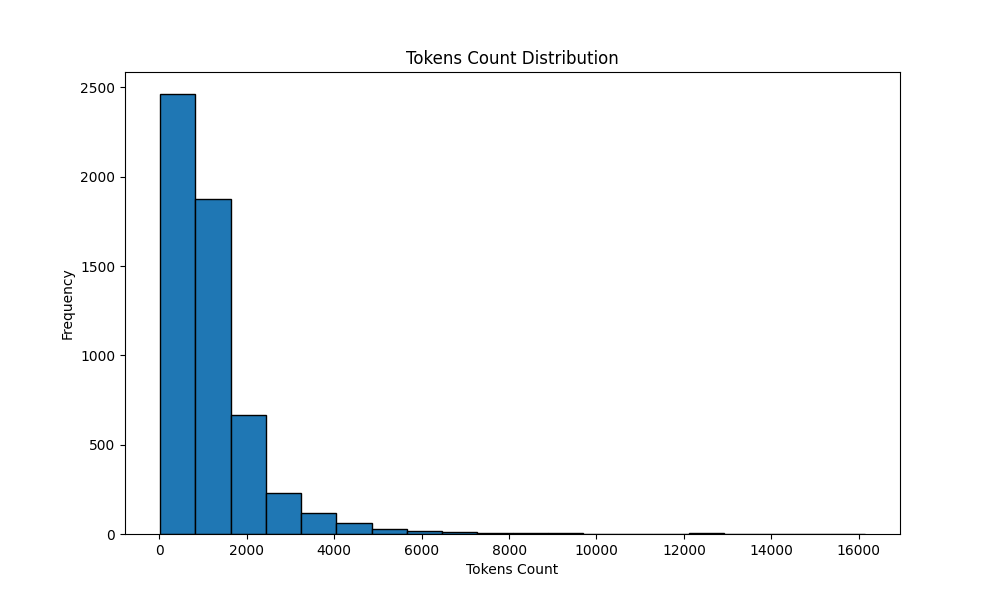
\includegraphics[width=0.9\linewidth]{figures/tokens_count_vx_hist.png}
    \caption{Articles token count distribution}
    \label{fig:tokens_hist}
\end{figure}

\begin{figure}[htbp]
    \centering
    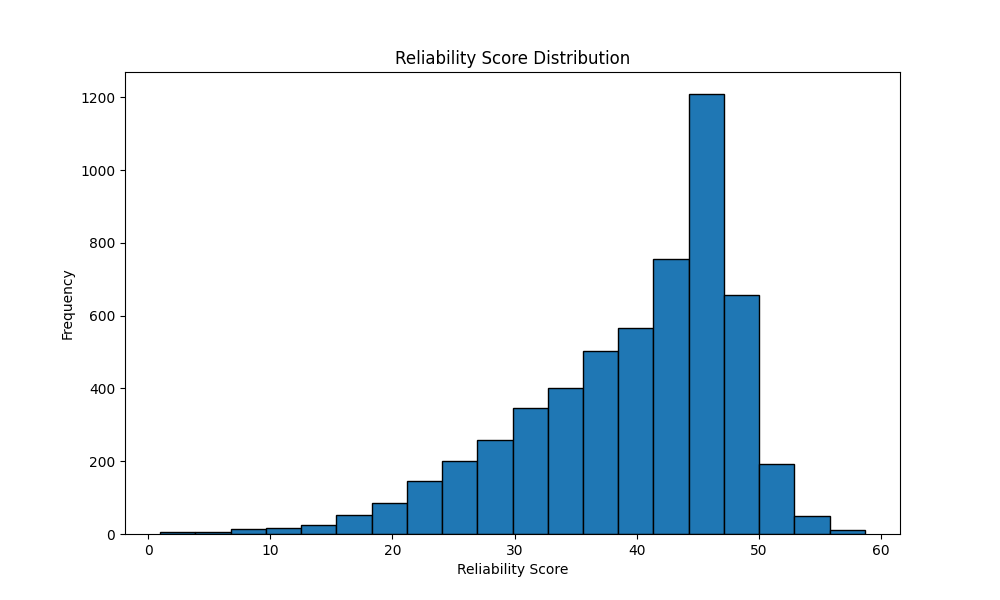
\includegraphics[width=0.9\linewidth]{figures/reliability_score_hist.png}
    \caption{Reliability score distribution}
    \label{fig:reliability_score_hist}
\end{figure}

Sub-words instead of words are used as tokens in this analysis. The length of article content tokens ranges from 17 to 16,139, with an average length of 1,207.07 and a median value of 908 tokens. Only 9 articles have more than 10,000 tokens, while 106 articles have fewer than 100 tokens. Furthermore, only 1,209 articles contain 512 tokens or fewer, which is the limit for BERT input. The articles' reliability scores range from 1.0 to 58.67, with the majority scoring between 20 and 50. No articles were rated higher than 60, despite the highest possible score being 64. Visualisations can be seen in both Figure \ref{fig:tokens_hist} and Figure \ref{fig:reliability_score_hist}, as well as Figure \ref{fig:tokens_hist_split}

\begin{figure}[htbp]
    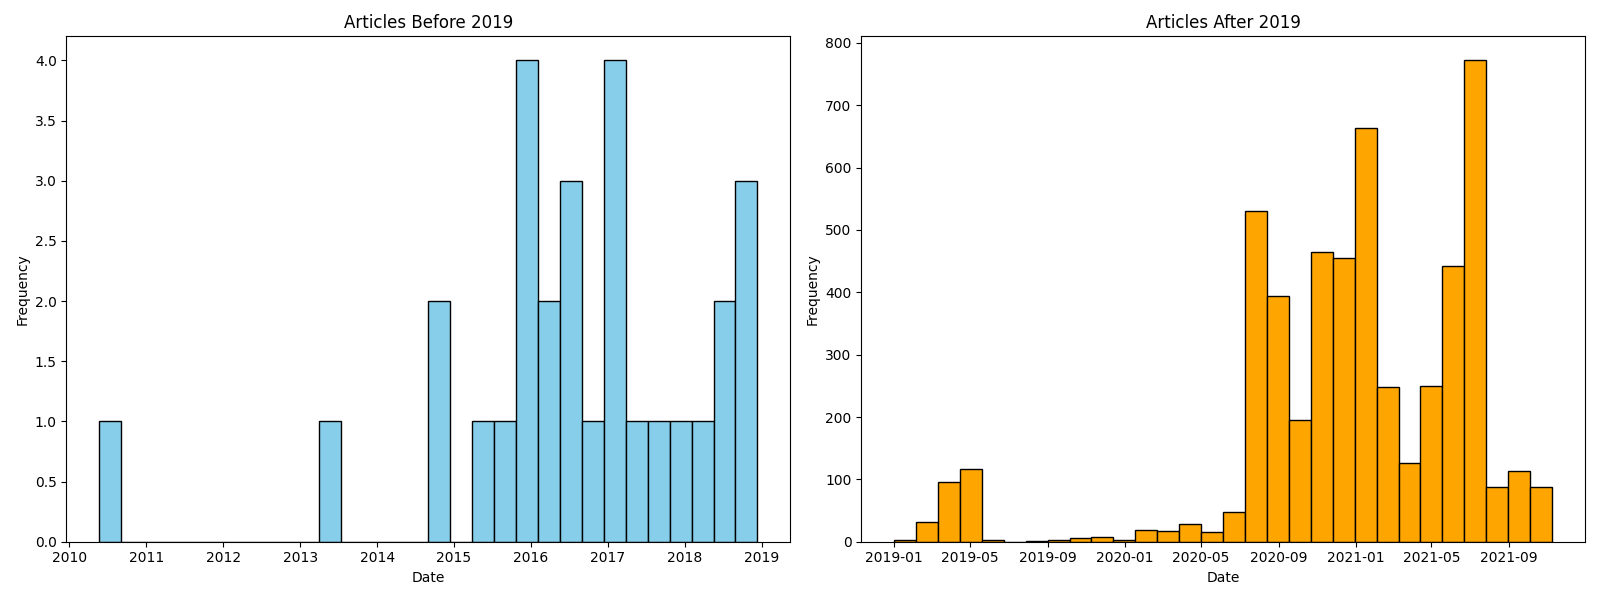
\includegraphics[width=0.9\linewidth]{figures/dates_hist.png}
    \caption{Article dates distribution}
    \label{fig:dates_hist}
\end{figure}

Most articles were written and published within the last six years, with only 31 articles published before 2019, as shown in Figure \ref{fig:dates_hist}. Looking at these 31 articles individually, they generally cover similar topics to those published after 2019 and therefore should not exhibit consequential differences in behaviour and characteristics.

\begin{figure}[htbp]
    \centering
    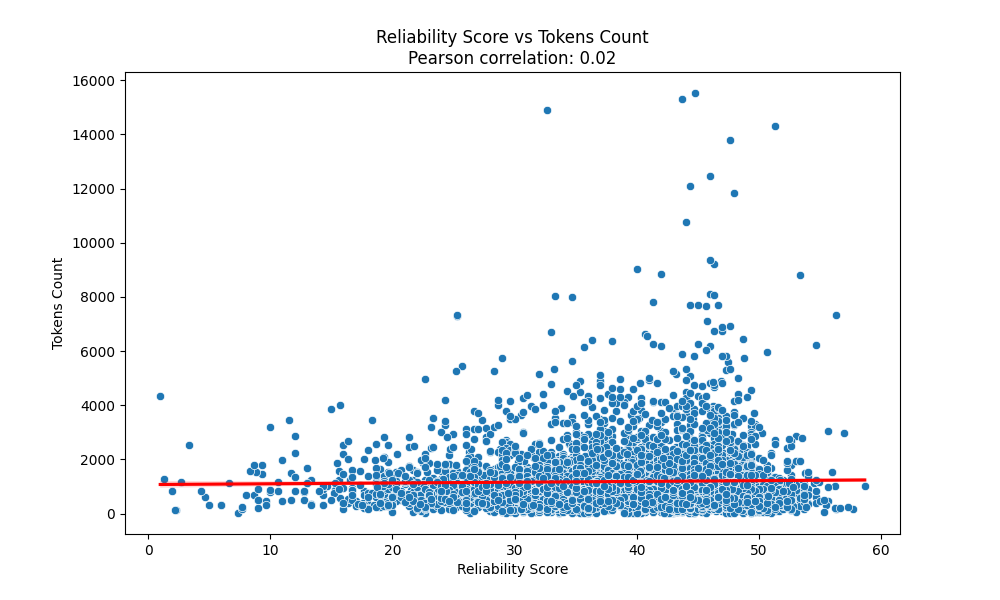
\includegraphics[width=0.9\linewidth]{figures/correlation_tokens_reliability_score.png}
    \caption{Pearson correlation between token count and reliability score}
    \label{fig:pearson_correlation}
\end{figure}


\begin{figure}[htbp]
    \centering
    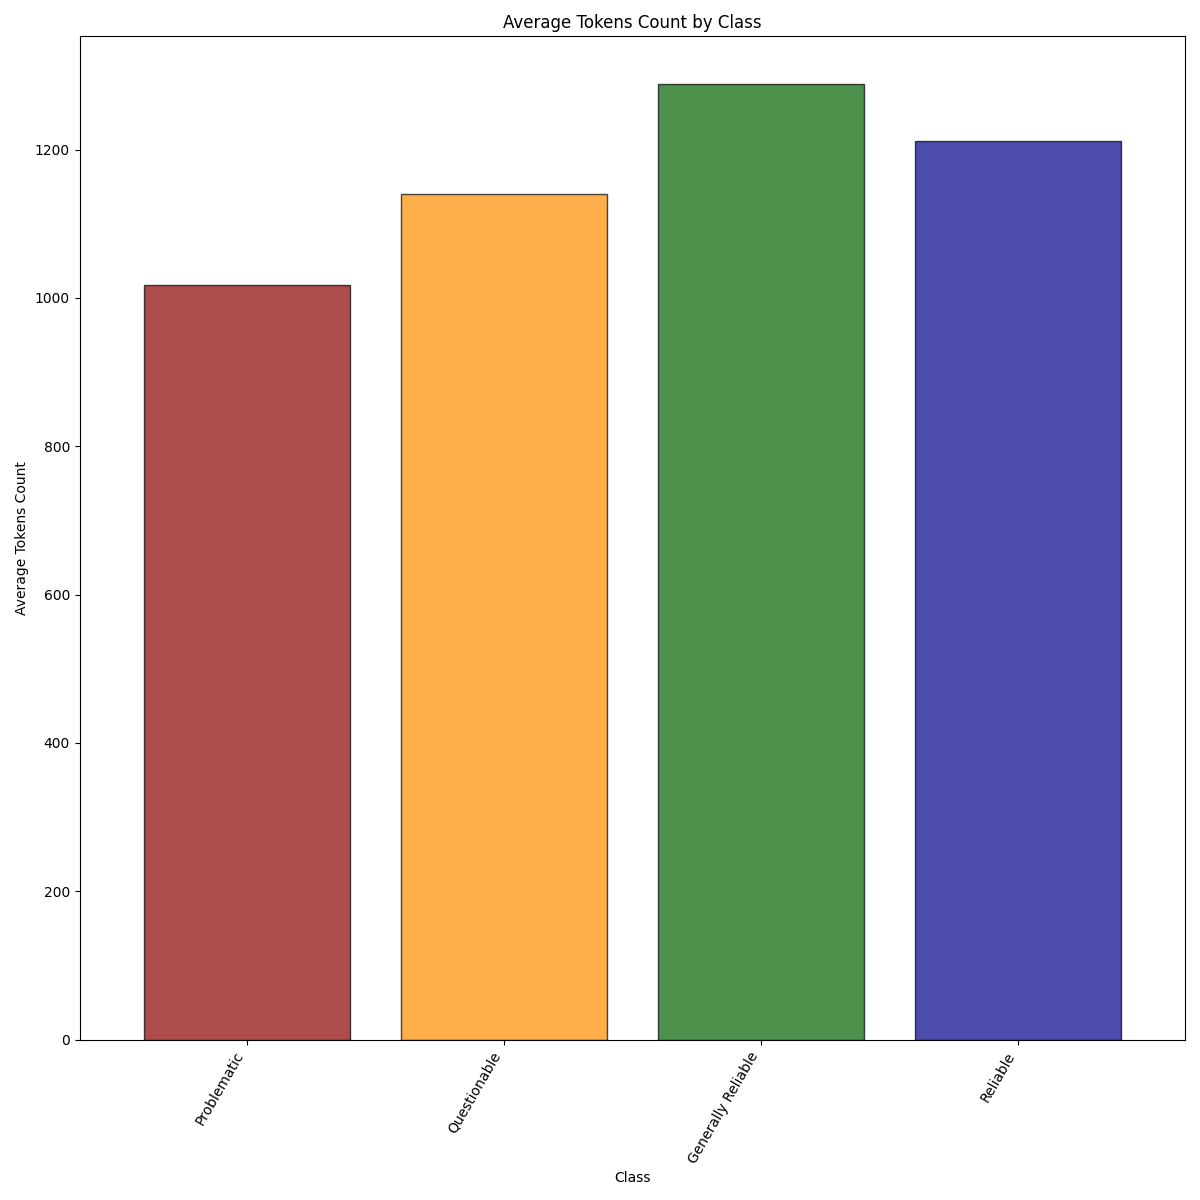
\includegraphics[width=0.8\linewidth]{figures/tokens_count_vx_per_class_hist.png}
    \caption{Average tokens count per class}
    \label{fig:avg_tokens_count_per_class}
\end{figure}

Figure \ref{fig:avg_tokens_count_per_class} shows that all classes have similar token counts, close to the overall average. The 'Problematic' and 'Questionable' classes, being the two most biased, have lower average token counts than the other two classes. Further analysis(Figure \ref{fig:pearson_correlation}) reveals that there is virtually no linear relationship between token count and reliability score, with a Pearson correlation coefficient of 0.02. This indicates that the length of an article has no significant impact on its reliability score. In other words, longer articles are not necessarily more or less reliable than shorter ones based on the provided data.

%%% Local Variables: 
%%% mode: latex
%%% TeX-master: "thesis"
%%% End: 